\begin{figure}
    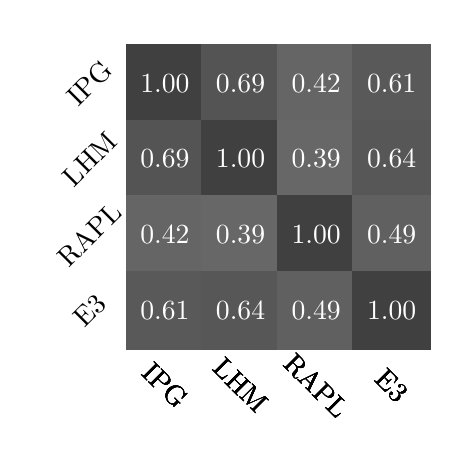
\begin{tikzpicture}[scale=0.6]
        \foreach \y [count=\n] in {{1.00, 0.69, 0.42, 0.61},{0.69, 1.00, 0.39, 0.64},{0.42, 0.39, 1.00, 0.49},{0.61, 0.64, 0.49, 1.00},} {
        % column labels
        \foreach \a [count=\n] in {IPG,LHM,RAPL,E3} {
          \node[minimum size=10mm, xshift=0.0cm, rotate=-45] at (\n*1.6, -8) {\a};
        }
        % heatmap tiles
        \foreach \x [count=\m] in \y {
          \pgfmathsetmacro{\xa }{(\x + 1) / 2 * 100}
          \node[fill=darkgray!\xa!lightgray, minimum size=10mm, text=white, font={\normalsize}] at (\m*1.6,-\n*1.6) {\x};
        }
      }
        % row labels
        \foreach \a [count=\i] in {IPG,LHM,RAPL,E3} {
          \node[minimum size=10mm, xshift=-0.0cm, yshift=-0.0cm, rotate=45] at (0,-\i*1.6) {\a};
        }
      \end{tikzpicture}
    \caption{This heat map represents Correlation coefficients between the different measuring instrument1 on the Surface Pro 4}
    \label{tab:HeatFasta}
\end{figure}